    \begin{enumerate}
        \item Le disque est en mouvement \textbf{rotation uniforme}
              \hfill\textbf{(0,5pt)} \\
              car il parcourt des arcs égaux pendant des durées égales
              ($\tau=\qty{40}{\ms}$).
              \hfill\textbf{(0,5pt)}
        \item $\ang{18}=18\times\frac{\pi}{180}=
              \frac{\pi}{10}~\unit{\rad}$ \\[2mm]
              $\omega_{3}=\frac{\theta_{4}-\theta_{2}}{2\tau}=
              \frac{\left(\frac{2\pi}{5}-\frac{\pi}{5}\right)}
              {2\times40\times10^{-3}}=
              \qty{7.85}{\radian\per\second}$
              \hfill\textbf{(1pt)}

        \item $v_{3}=R\times\omega_{3}=3\times10^{-2}\times7,85=\qty{0.236}{\v}$
              \hfill\textbf{(1pt)}
        \item 
              $\qty{0.236}{\v} \to \qty{2.36}{\cm}$.
              \hfill\textbf{(0,5pt)}

        \begin{figure}[H]
            \centering
            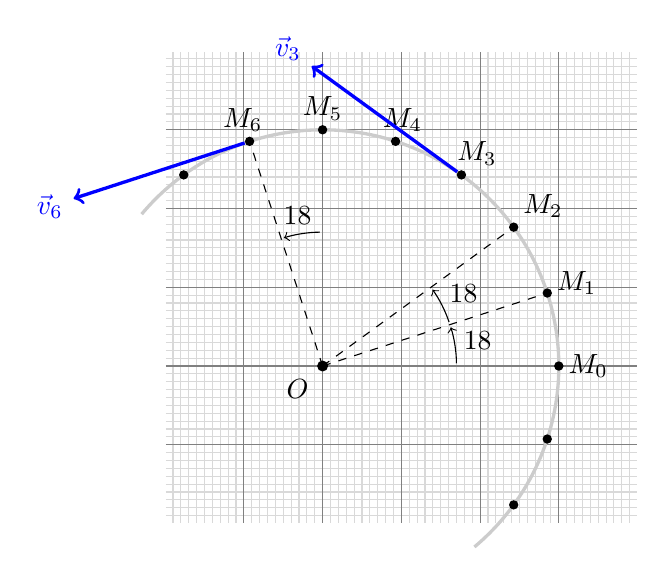
\begin{tikzpicture}
                \def\th{18}
                \newdimen\r \r=3cm
                \draw[step=1mm,black!15] (-1.99,-1.99) grid (3.99,3.99);
                \draw[step=1cm,black!50] (-1.99,-1.99) grid (3.99,3.99);
                \node[inner sep=1.4pt,circle,fill,label=below left:$O$] {};
                \draw[black!20,very thick] (140:\r) arc (140:-50:\r);
                \foreach \a [count=\i from 0] in {0,18,...,140,-36,-18,...,-1}
                    \node[circle,inner sep=1.2pt,fill] (M\i) at (\a:\r) {};
                \foreach \i in {0,...,6}
                    \node[anchor=180+\i*\th] at (M\i) {$M_{\i}$};
                \draw[dashed] (0,0) -- (M1) (0,0) -- (M2) (0,0) -- (M6);
                \foreach \a in {0, \th, 90}
                    \draw[->,shorten <=1pt,shorten >=1pt] (\a:1.7) arc (\a:\a+\th:1.7)
                        node[anchor=180+\a,pos=0.6] {$\qty{18}{\degree}$};
                % corr
                \draw[->,very thick,blue] (M3) -- ++(90+3*\th:2.35)
                    node[anchor=-90+3*\th] {$\vec{v}_{3}$};
                \draw[->,very thick,blue] (M6) -- ++(90+6*\th:2.35)
                    node[anchor=-90+6*\th] {$\vec{v}_{6}$};
            \end{tikzpicture}
        \end{figure}
        
    \end{enumerate}
